\subsection{Accelerometer}

The primary motivation for including a wearable in the system is to access the accelerometer and use its acceleration data to perform gesture recognition.

Accelerometers are used for measuring the acceleration of an object. In our case we use it to measure the acceleration of the wearable installed on a users wrist and as a result of this, the users arm movements. When measuring the users movements, we can recognize the gestures he performs.

When an object is subjected to a force, including gravity, it accelerates. Acceleration can be expressed as change in velocity over time as in \Cref{eq:acceleration-delta-velocity} where $\vec{a}$ is the acceleration, $\Delta v$ is the change in velocity and $\Delta t$ is the duration.
Velocity is measured as meters per second and time is measured in seconds, hence the acceleration is measured as meters per second or $\frac{m}{s^2}$.
Acceleration can also be expressed in terms of force applied to the object as in \Cref{eq:acceleration-force} where $a$ is the acceleration of the object, $F$ is the forces applied to the object expressed as a vector with a force for each axis and $m$ is the mass expressed as a scalar value.
The forces are measured in Newton and mass is measured in kg.

\begin{centering}
\begin{minipage}{.5\linewidth}
    \begin{equation}
    \vec{a} = \frac{\Delta v}{\Delta t}
    \label{eq:acceleration-delta-velocity}
    \end{equation}
\end{minipage}
\begin{minipage}{.5\linewidth}
    \begin{equation}
    a = \frac{F}{m}
    \label{eq:acceleration-force}
    \end{equation}
\end{minipage}
\end{centering}

The accelerometer determines the force applied to the object~\cite[pp. 392-393]{Fraden:2112745} so in order to calculate the acceleration, the mass of the object must be known.

Accelerometers of varying design exist~\cite[pp. 392-411]{Fraden:2112745}. An example of these is the capacitive type semiconductor accelerometer which is illustrated in \Cref{fig:accelerometer}. The accelerometer has an electrode in the middle (14) which is supported by a beam (13). The beam is flexible enough to move slightly up and down when the accelerometer is moved, thus moving the electrode up and down. The beam is mounted to the side of the accelerometer (2). The gap between the electrode (14) and the two stationary electrodes (25, 26) constitute two electric capacitors having capacitances of $C_1$ and $C_2$.
When the movable electrode in the middle (14) moves up and down, the capacitances $C_1$ and $C_2$ changes slightly~\cite{kloeck1993capacitive}.

The changes are registered and constitutes the acceleration. This allows for measuring the acceleration on one axis. The same principle can be used to measure the acceleration on several axes.

In this project we utilize the accelerometer for recognizing gestures but other common applications of the accelerometer include pedometers, game controllers and fall detection.

\begin{figure}
\centering
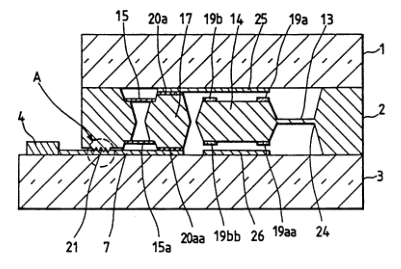
\includegraphics[width=0.5\textwidth]{images/accelerometer}
\caption{Capacitive type semiconductor accelerometer~\cite{kloeck1993capacitive}.}
\label{fig:accelerometer}
\end{figure}

%%% Local Variables:
%%% mode: latex
%%% TeX-master: "../../master"
%%% End:
